\documentclass[12pt]{article}
\usepackage[utf8]{inputenc}
\usepackage{latexsym,amsfonts,amssymb,amsthm,amsmath}
\usepackage{float}
\usepackage{caption}
\usepackage{marginnote}
\usepackage{tikz}
\usepackage{hyperref}

\setlength{\parindent}{0in}
\setlength{\oddsidemargin}{0in}
\setlength{\textwidth}{6.5in}
\setlength{\textheight}{8.8in}
\setlength{\topmargin}{0in}
\setlength{\headheight}{18pt}

\newtheorem*{answer*}{Answer}
\newtheorem*{solution*}{Solution}
\newtheorem{remark}{Remark}

\title{Weekly Homework 31}
\author{Math Gecs}
\date{October 06, 2024}

\begin{document}
\maketitle

\subsection*{Exercise 1}
We consider a fixed point $P$ in the interior of a fixed sphere$.$ We construct three segments $PA, PB,PC$, perpendicular two by two$,$ with the vertexes $A, B, C$ on the sphere$.$ We consider the vertex $Q$ which is opposite to $P$ in the parallelepiped (with right angles) with $PA, PB, PC$ as edges$.$ Find the locus of the point $Q$ when $A, B, C$ take all the positions compatible with our problem.\\

Source: 1978 IMO Problem 2\\


\begin{solution*}

Let $R$ be the radius of the given fixed sphere.
\begin{figure}[H]
    \centering
    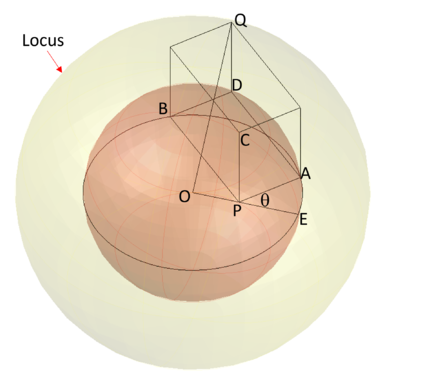
\includegraphics[width=8cm]{locus.png}
    \label{fig:node-1}
\end{figure}
Let point $O$ be the center of the sphere.

Let point $D$ be the 4th vertex of the face of the parallelepiped that contains points $P$, $A$, and $B$.

Let point $E$ be the point where the line that passes through $OP$ intersects the circle on the side nearest to point $A$

Let $\alpha=\angle AOP,\;\beta=\angle BPD,\;\theta=\angle APE$

We start the calculations as follows:

$\left| AB \right|= \left| PD \right|$

$\left| AB \right|^{2}=\left| PA \right|^{2}+\left| PB \right|^{2}$

Therefore, $\left| PD \right|^{2}=\left| PA \right|^{2}+\left| PB \right|^{2}$ [Equation 1]

Using law of cosines:

$R^{2}=\left| OP \right|^{2} + \left| PB \right|^{2} - 2 \left| OP \right| \left| PB \right| cos (\angle OPB)$

$R^{2}=\left| OP \right|^{2} + \left| PB \right|^{2} - 2 \left| OP \right| \left| PB \right| cos \left( \frac{\pi}{2}-\theta \right)$

$R^{2}=\left| OP \right|^{2} + \left| PB \right|^{2} - 2 \left| OP \right| \left| PB \right| sin (\theta)$

$\left| PB \right|^{2} =R^{2}-\left| OP \right|^{2} + 2 \left| OP \right| \left| PB \right| sin (\theta)$ [Equation 2]

Using law of cosines again we also get:

$\left| PA \right|^{2} =R^{2}+\left| OP \right|^{2} - 2 \left| OP \right| R cos(\alpha)$

Since $R cos(\alpha) = \left| PA \right| cos(\theta) + \left| OP\right|$, then

$\left| PA \right|^{2} =R^{2}+\left| OP \right|^{2} - 2 \left| OP \right| \left[ \left| PA \right| cos(\theta) + \left| OP\right| \right]$

$\left| PA \right|^{2} =R^{2}-\left| OP \right|^{2} - 2 \left| OP \right| \left| PA \right| cos(\theta)$ [Equation 3]

Substituting [Equation 2] and [Equation 3] into [Equation 1] we get:

$\left| PD \right|^{2}=2R^{2}-2\left| OP \right|^{2}+2\left| OP \right| \left[ \left| PB \right| sin(\theta) - \left| PA \right| cos(\theta) \right]$ [Equation 4]

Now we apply the law of cosines again:

$\left| OD \right|^{2}=\left| OP \right|^{2}+\left| PD \right|^{2}-2\left| OP \right| \left| PD \right|cos(\angle OPD)$

$\left| OD \right|^{2}=\left| OP \right|^{2}+\left| PD \right|^{2}-2\left| OP \right| \left| PD \right| cos(\angle OPB+\angle BPD)$

$\left| OD \right|^{2}=\left| OP \right|^{2}+\left| PD \right|^{2}-2\left| OP \right| \left| PD \right| cos \left(\frac{\pi}{2}-\theta+\beta \right)$

$\left| OD \right|^{2}=\left| OP \right|^{2}+\left| PD \right|^{2}-2\left| OP \right| \left| PD \right| sin(\theta-\beta)$

$\left| OD \right|^{2}=\left| OP \right|^{2}+\left| PD \right|^{2}-2\left| OP \right| \left| PD \right| \left[sin(\theta)cos(\beta)-sin(\beta)cos(\theta)  \right]$

Since, $sin(\beta)=\frac{\left| PA \right|}{\left| PD \right|}$ and $cos(\beta)=\frac{\left| PB \right|}{\left| PD \right|}$ then,

$\left| OD \right|^{2}=\left| OP \right|^{2}+\left| PD \right|^{2}-2\left| OP \right| \left| PD \right| \left[\frac{\left| PB \right|}{\left| PD \right|}sin(\theta)-\frac{\left| PA \right|}{\left| PD \right|}cos(\theta)  \right]$

$\left| OD \right|^{2}=\left| OP \right|^{2}+\left| PD \right|^{2}-2\left| OP \right| \left[\left| PB \right|sin(\theta)-\left| PA \right|cos(\theta)  \right]$ [Equation 5]

Substituting [Equation 4] into [Equation 5] we get:

$\left| OD \right|^{2}=\left| OP \right|^{2}+2R^{2}-2\left| OP \right|^{2}+2\left| OP \right| \left[ \left| PB \right| sin(\theta) - \left| PA \right| cos(\theta) \right]-2\left| OP \right| \left[\left| PB \right|sin(\theta)-\left| PA \right|cos(\theta)  \right]$

Notice that all of the terms with $\theta$ cancel and thus we're left with:

$\left| OD \right|^{2}=2R^{2}-\left| OP \right|^{2}$ regardless of $\theta$. [Equation 6]

Now we need to find $\left| PC \right|$

Since points $O$, $P$, and $C$ are on the plane perpendicular to the plane with points $O$, $P$, and $A$, then these points lie on the big circle of the sphere. Therefore the distance $\left| PC \right|$ can be found using the formula:

$R^{2}=\left| OP \right|^{2}+\left| PC \right|^2$

Solving for $\left| PC \right|^2$ we get:

$\left| PC \right|^2=R^{2}-\left| OP \right|^{2}$ [Equation 7]

Now we need to get $\left| OQ \right|^{2}$ which will be using the formula:

$\left| OQ \right|^{2}=\left| OD \right|^{2}+\left| PC \right|^2$ [Equation 8]

Substituting [Equation 6] and [Equation 7] into [Equation 8] we get:

$\left| OQ \right|^{2}=2R^{2}-\left| OP \right|^{2}+R^{2}-\left| OP \right|^{2}$

This results in:

$\left| OQ \right|^{2}=3R^{2}-2\left| OP \right|^{2}$

which is constant regardless of $\theta$ and constant regardless of where points $A$, $B$, and $C$ are located as long as they're still perpendicular to each other.

In space, this is a sphere with radius $\left| OQ \right|$ which is equal to $\sqrt{3R^{2}-2\left| OP \right|^{2}}$

Therefore, the locus of vertex $Q$ is a sphere of radius $\sqrt{3R^{2}-2\left| OP \right|^{2}}$ with center at $O$, where $R$ is the radius of the given sphere and $\left| OP \right|$ the distance from the center of the given sphere to point $P$
\end{solution*}



\end{document}